\documentclass{beamer}

\usetheme{src/sintef}
\usefonttheme[onlymath]{serif}
% \titlebackground*{beamerthemesrc/assets/background}
%-------------add your packages here-------------
\usepackage{amsfonts,amsmath,oldgerm}

%-------------add your commands here-------------
\newcommand{\hrefcol}[2]{\textcolor{cyan}{\href{#1}{#2}}}
\newcommand{\testcolor}[1]{\colorbox{#1}{\textcolor{#1}{test}}~\texttt{#1}}




%-------------title here--------------------
\title{Load Balancer e API Gateway}
\subtitle{}
\course{}
\author{Ramon Santos}
\IDnumber{}

%--------------begin document--------------------
\begin{document}
\maketitle


\section{Camadas de redes no modelo TCP/IP}
\begin{frame}[fragile]{Camadas de redes no modelo TCP/IP}
    \begin{itemize}%[<+->]
        \item Camada de aplicação:
            \begin{itemize}%[<+->]
                \item contém os protocolos de alto nível;
                \item HTTP, DNS, SMTP, FTP e etc.
            \end{itemize}
        \item Camada de transporte:
            \begin{itemize}%[<+->]
                \item responsável pela comunicação end-to-end entre dois dispositivos;
                \item recebe dados da camada de aplicação, os divide em unidades menores e repassa para a camada de rede;
                \item TCP e UDP.
            \end{itemize}
    \end{itemize}
\end{frame}

\begin{frame}[fragile]{Camadas de redes no modelo TCP/IP}
    \begin{itemize}%[<+->]
        \item Camada de internet (ou camada de rede):
            \begin{itemize}%[<+->]
                \item faz o roteamento de pacotes entre diferentes redes;
                \item IP e ICMP.
            \end{itemize}
        \item Camada de enlace:
            \begin{itemize}%[<+->]
                \item lida com a comunicação física entre os dispositivos;
                \item Ethernet (via cabo), 802.11 (sem fio) e etc.
            \end{itemize}
    \end{itemize}
\end{frame}


\section{Proxy de encaminhamento vs proxy reverso}
\begin{frame}[fragile]{Forward Proxy (encaminhamento)}
    \begin{itemize}%[<+->]
        \item Atua entre o cliente e a internet É usado para controle de acesso, filtragem de conteúdo, anonimato e cache.\newline
        
        \begin{figure}
            \centering
            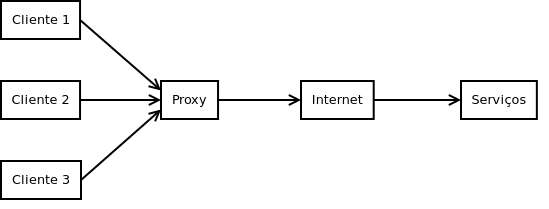
\includegraphics[width=0.7\linewidth]{contents//img/1.png}
            \caption{Forward proxy}
            \label{fig:enter-label}
        \end{figure}

    \end{itemize}
\end{frame}

\begin{frame}[fragile]{Proxy reverso}
    \begin{itemize}%[<+->]
        \item Um proxy reverso é um servidor que recebe as requisições dos clientes e as redireciona para os servidores de backend apropriados. \newline
        
        \begin{figure}
            \centering
            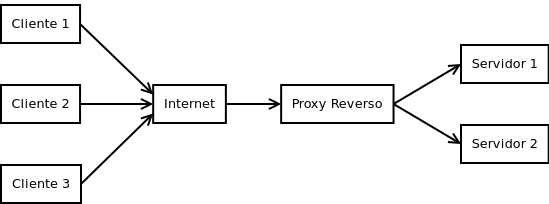
\includegraphics[width=0.7\linewidth]{contents//img/2.png}
            \caption{Proxy reverso}
            \label{fig:enter-label}
        \end{figure}
    \end{itemize}
\end{frame}

\section{Load balancer}
\begin{frame}[fragile]{Load balancing}
    \begin{itemize}%[<+->]
        Load balancing (balanceamento de carga) é o processo de redistribuição da carga de trabalho entre os nós de um sistema distribuído para melhorar tanto a utilização dos recursos, quanto o tempo de resposta das tarefas, evitando também situações em que alguns nós fiquem muito carregados enquanto outros fiquem ociosos ou realizando pouco trabalho.
    \end{itemize}
\end{frame}


\begin{frame}[fragile]{Características de um load balancing}
    \begin{itemize}%[<+->]
        \item Distribuir tráfego/carga entre múltiplos servidores.
        \item Possibilita a escalabilidade horizontal.
        \item Segurança: Separa tráfego público de tráfego privado.
        \item Pode atuar nas camadas de aplicação e transporte.
        \item Realizam health checks para verificar se um servidor consegue receber requisições.
        \item Possibilita manutenção de servidores sem downtime.
    \end{itemize}
\end{frame}


\begin{frame}[fragile]{Mecanismos de balanceamento}
    \begin{itemize}%[<+->]
        \item \textbf{Round Robin:} Envia requisições sequencialmente entre os servidores.
        \item \textbf{Least Connections:} Escolhe o servidor com menos conexões ativas.
        \item \textbf{IP Hash:} Uma função hash é usada para determinar qual servidor deve receber a próxima request com base no endereço IP do cliente.
        \item \textbf{Weighted load balancing:} Usa o algoritmo Round Robin com diferentes pesos nos servidores. É útil quando determinado servidor conta com mais capacidade computacional que os demais.
        \item \textbf{Least Time:} Escolhe o servidor com o menor tempo médio de resposta.
    \end{itemize}
\end{frame}

\begin{frame}[fragile]{Ferramentas}
    \begin{itemize}%[<+->]
        \item \textbf{Nginx:} Leve e extensível (com Lua). Muito usado para balancear carga HTTP.
        \item \textbf{HAProxy:} Além de ser usado para balanceamento de carga na camada de aplicação, é bastante popular no balanceamento de carga na camada de transporte. Como, por exemplo, balanceamento de conexão de leitura entre réplicas read-only do PostgreSQL.
        \item \textbf{Cloudflare Load Balancing:} É um serviço de balanceamento de carga global, que tem como principal característica o um roteamento inteligente e personalizável, onde a região geográfica, ou até mesmo as coordenadas do GPS do dispositivo que fez a requisição, podem ser considerados para encontrar o nó de menor latência.
        \item \textbf{AWS Elastic Load Balancing:}
        \begin{itemize}
            \item \textbf{Application Load Balancer:} Balanceador de carga da camada de aplicação.
            \item \textbf{Network Load Balancer:} Balanceador de carga da camada de transporte.
        \end{itemize}
    \end{itemize}
\end{frame}

\section{API Gateway}
\begin{frame}[fragile]{API Gateway}
    \begin{itemize}%[<+->]
        Um API Gateway é um ponto de entrada único para gerenciar e encaminhar requisições a diferentes serviços de uma aplicação em um sistema distribuído.
    \end{itemize}
\end{frame}


\begin{frame}[fragile]{Características de um API gateway}
    \begin{itemize}%[<+->]
        \item Pode fazer balanceamento de carga.
        \item Atua na camada de aplicação.
        \item Faz tradução de protocolo.
        \item Monitoramento, Logging e Analytics.
        \item Gerenciamento da API:
            \begin{itemize}
                \item roteia requisições para serviços mapeados;
                \item versionamento de API;
                \item adiciona headers e query params;
                \item throttling e rate limiting;
                \item transformação e agregação de resposta.
            \end{itemize}
        \item Diminui carga de trabalho nos serviços:
            \begin{itemize}
                \item pode responder a requisições com dados em cache;
                \item pode lidar com autenticação e autorização;
                \item validação de requisições;
                \item não repassaria requisições de um ataque DDoS para serviços.
            \end{itemize}
    \end{itemize}
\end{frame}


\begin{frame}[fragile]{Desafios e desvantagens}
\begin{itemize}%[<+->]
        \item Adiciona uma nova camada da arquitetura:
            \begin{itemize}
                \item mais um componente para o time manter;
                \item mais ferramentas que as pessoas do time devem conhecer;
                \item cada request passa por uma nova camada, o que pode gerar latência adicional;
                \item aumenta o custo financeiro com ferramentas gerenciadas ou infra em soluções self-hosted.
            \end{itemize}
        \item É um ponto único de falha:
            \begin{itemize}
                \item se o gateway cair, todos os serviços ficam inoperantes;
                \item erros de configuração podem comprometer segurança e desempenho;
                \item é necessário buscar alta disponibilidade, mediante técnicas como replicação e balanceamento, ou usar serviços gerenciados que suportem esse requisito.
            \end{itemize}
    \end{itemize}
\end{frame}

\begin{frame}[fragile]{Ferramentas}
    \begin{itemize}%[<+->]
        \item \textbf{Kong:} Funciona com Nginx e é extensível através de plugins escritos em Lua.
        \item \textbf{AWS API Gateway:} Serviço de API Gateway gerenciado da AWS.
    \end{itemize}
\end{frame}

\section{Referências}
\begin{frame}[fragile]{Referências}
    \begin{itemize}%[<+->]
        \item \textbf{Documentação no Nginx sobre load balancer:} https://docs.nginx.com/nginx/admin-guide/load-balancer/http-load-balancer/
        \item \textbf{Capítulo 20 do Livro \textit{Engenharia de Confiabilidade do Google}:} (Existe a versão em português do livro pela Novatec e o livro está disponível de graça em inglês neste link https://sre.google/sre-book/table-of-contents/).
        \item \textbf{Post sobre API Gateway \textit{What Is an API Gateway?}:} https://www.paloaltonetworks.co.uk/cyberpedia/what-is-api-gateway
    \end{itemize}
\end{frame}



\backmatter
\end{document}
